\documentclass[11pt]{article}

\usepackage[margin=1in]{geometry}
\usepackage{booktabs}
\usepackage{hyperref}
\usepackage{natbib}
\usepackage{graphicx}
\usepackage{array}
\usepackage{longtable}
\usepackage{microtype}

\title{FreightBidBench: Feasibility Calibration for Public Real-Time Truckload Bid Benchmarks\thanks{Code and benchmark artifacts: \url{https://github.com/aswincsekar/freightbidbench} (release \texttt{v0.2.1}, commit \texttt{c0a385c1e269afe4efa4cfa1ca9afa6e7d37ca14}).}}
\author{Aswin Chandrasekaran}
\date{Draft v0.2.1 -- May 9, 2026}

\begin{document}
\maketitle

\begin{abstract}
Truckload carriers and brokers make accept/reject decisions under tight
latency, uncertain future demand, and operational feasibility constraints.
Existing academic formulations often study dynamic fleet management or
stochastic vehicle routing, but public benchmarks for real-time truckload bid
evaluation rarely combine stochastic tenders, closed-loop fleet state, latency
measurement, and driver/facility feasibility. We introduce FreightBidBench, a
public-calibrated synthetic benchmark built from FAF freight-flow structure and
USDA AMS truck-rate reports. Version 0.2 adds individual truck state, pickup
reach time, pickup and delivery appointment windows, simplified
hours-of-service clocks, and stochastic shipper/receiver yard delays. The main
empirical finding is calibrative: removing appointment windows raises myopic
profit by 124 percent in \texttt{tight} and 194 percent in \texttt{scarce}, and
removing HOS raises myopic profit by 116 percent and 155 percent in the same
scenarios; disabling the full feasibility stack raises \texttt{scarce} myopic
profit by 219 percent. At the same time, simple feasible or myopic policies
remain near the finite rollout teacher in the full-feasibility benchmark. Thus,
v0.2 shows that operational feasibility is a first-order benchmark object for
online accept/reject decisions evaluated with closed-loop fleet state and
latency, not bookkeeping.
\end{abstract}

\section{Introduction}

Real-time truckload bid acceptance is a high-pressure sequential decision
problem. A carrier can accept a load that looks profitable immediately but
sends a truck into a weak future market, violates pickup feasibility, or
consumes driver hours needed for a better future load. Conversely, rejecting a
low-margin load can be costly when the destination improves fleet positioning.

The main obstacle to reproducible research in this setting is not only model
choice. It is also measurement. A benchmark that omits pickup reach,
appointment windows, HOS clocks, or yard delays can make a fast policy look
strong for the wrong reason: it is not being charged for the operational work
needed to make the acceptance decision real. Private tender data is rarely
shareable, and production dispatch systems are complex and unavailable to most
researchers, so this measurement problem is hard to audit.

FreightBidBench addresses this gap with a public-calibrated benchmark rather
than a claim of production-grade simulation. The purpose is to create a common
testbed where researchers can compare policies on the same stochastic freight
environment and report the same profit, latency, and feasibility metrics.

This paper uses FreightBidBench v0.2 as a calibration study. The headline is
not that v0.2 produces a clean latency-quality frontier. It does not. Instead,
v0.2 shows that feasibility constraints dominate the interpretation of policy
results, and that additional economic and temporal structure is needed before a
future version should be used to rank sophisticated acceleration methods.

\section{Contributions}

This paper makes six contributions.

\begin{enumerate}
  \item We introduce FreightBidBench, a reproducible public-calibrated
  benchmark for real-time truckload bid acceptance.
  \item We define a closed-loop synthetic freight environment calibrated from
  public FAF and USDA-derived inputs.
  \item We add a v0.2 feasibility layer with individual trucks, pickup reach
  time, pickup and delivery appointment windows, simplified HOS clocks, and
  stochastic yard delays.
  \item We show that removing appointment windows or HOS can more than double
  myopic profit in tight and scarce scenarios, showing that these constraints
  are first-order relative to the policy gaps observed in v0.2.
  \item We report reference policies, paired-seed policy differences, latency,
  and feasibility metrics under a manifest-based reproducibility contract.
  \item We diagnose why v0.2 is a calibration benchmark rather than a final
  latency-frontier benchmark: accepted-but-unserviceable tenders are
  under-penalized, terminal truck position has weak carryover value, temporal
  demand structure is limited, and the rollout teacher is not an upper bound.
  We identify a realized-seed hindsight optimization bound as the next
  diagnostic ceiling for v0.3.
\end{enumerate}

\section{Related Work}

\paragraph{Dynamic truckload acceptance and fleet management.}
Dynamic truckload routing and load acceptance has long been recognized as an
online, state-dependent decision problem. Kim, Mahmassani, and Jaillet study
dynamic load acceptance and rejection decisions for large-fleet truckload
operations with time windows and priority demand \citep{kim2004dynamic}.
Simao et al. show how approximate dynamic programming can estimate marginal
driver values in large-scale truckload fleet management \citep{simao2009adp}.
FreightBidBench builds on this tradition but changes the artifact: instead of
proposing one dispatch method, it provides a benchmark where future-value
policies, rollout teachers, and fast approximations can be compared under the
same stochastic seeds and latency measurements.

\paragraph{Dynamic and stochastic vehicle routing.}
Surveys by Pillac et al. and Ritzinger et al. describe the broader dynamic and
stochastic vehicle-routing literature, including the role of information
evolution and the distinction between online computation and offline policy
construction \citep{pillac2013review,ritzinger2016survey}. Ulmer et al.
combine offline value function approximation with online rollout for dynamic
routing with stochastic requests \citep{ulmer2019offline}, while Ulmer and
Thomas study value-function approximations for dynamic customer acceptance in
delivery routing \citep{ulmer2020meso}. These papers motivate
FreightBidBench's finite rollout teacher and surrogate baselines. The
benchmark gap is that truckload bid evaluation also requires public
calibration, fleet repositioning, operational feasibility, and latency-profit
reporting.

\paragraph{Routing benchmark instances.}
Classical public routing benchmarks such as Solomon's VRPTW instances and the
larger Homberger-Gehring VRPTW instances made vehicle-routing algorithms
comparable across papers \citep{solomon1987vrptw,homberger2005vrptw}.
FreightBidBench follows that reproducibility tradition, but the object is
different. Static VRPTW instances evaluate route construction for a known
customer set; FreightBidBench evaluates online accept/reject decisions where
accepted loads change truck positions, consume driver clocks, interact with
future stochastic tenders, and must be scored with decision latency and
feasibility diagnostics.

\paragraph{Adjacent dynamic benchmarks and public mobility testbeds.}
Public urban mobility studies have used taxi trip data to evaluate
shareability networks and large-scale dynamic trip-vehicle assignment
\citep{santi2014shareability,alonsomora2017ondemand}. Recent stochastic VRP
benchmarks such as SVRPBench move closer to benchmark artifacts for uncertain
urban logistics by releasing constraint-rich instances with stochastic travel
conditions and time windows \citep{heakl2025svrpbench}. FreightBidBench is
complementary: it targets truckload tender acceptance rather than passenger
pooling or parcel routing, with long-haul origin/destination freight flows,
accept/reject economics, individual tractor state, HOS clocks, pickup/delivery
appointments, and decision-latency reporting.

\paragraph{Learning-augmented optimization.}
Recent work uses learned models to speed up routing and stochastic
optimization. Nazari et al. and Kool et al. show that neural policies can
learn routing heuristics with fast inference after training
\citep{nazari2018rlvrp,kool2019attention}. Patel et al. approximate expensive
two-stage stochastic-programming value functions with neural surrogates
\citep{patel2022neur2sp}. Derrow-Pinion et al. demonstrate graph neural
networks for large-scale transportation ETA prediction
\citep{derrowpinion2021eta}. These works support future FreightBidBench
submissions, but the benchmark contribution is not a neural architecture. It is
a reproducible environment and reporting protocol for closed-loop truckload bid
evaluation.

\paragraph{Public freight data and feasibility rules.}
FreightBidBench uses the Freight Analysis Framework as a public freight-flow
backbone \citep{btsfaf5} and USDA AMS Specialty Crops National Truck Rate
Reports for refrigerated truck-rate and availability signals
\citep{usdafvwtrk}. The v0.2 feasibility layer uses a simplified
property-carrying HOS abstraction based on FMCSA's 11-hour driving limit,
14-hour driving window, and 10-hour off-duty reset summary \citep{fmcsa_hos}.
These data sources make the benchmark reproducible while also defining its
limits: the generated tenders are synthetic and public-calibrated, not private
carrier histories.

\section{Benchmark Design}

\subsection{Decision Problem}

At each decision epoch, the environment tenders a candidate load. A policy
chooses accept or reject. If accepted, the benchmark attempts to assign a
feasible truck. If no feasible truck exists, the accepted load creates a
no-truck or infeasible outcome. If feasible, the truck moves to the destination
and becomes available after pickup, linehaul, delivery, yard delays, and
required HOS rest.

\subsection{State}

The v0.2 state includes the candidate load origin/destination, load price,
direct cost, lane distance, public-calibrated lane intensity, state-level
future-value features, individual truck locations, truck availability times,
simplified HOS drive and duty clocks, pickup and delivery appointment windows,
pickup deadhead time, and yard-delay realizations.

\subsection{Reward}

For accepted feasible loads, profit is
\[
  \mathrm{profit} = \mathrm{price} - \mathrm{direct\ cost}
  - \mathrm{pickup\ deadhead\ cost} - \mathrm{yard\ delay\ cost}.
\]
Rejected loads receive zero immediate reward and preserve fleet state.

\section{Public Calibration}

FreightBidBench uses FAF state-level freight flows to seed
origin-destination intensity and regional imbalance. It uses USDA AMS FVWTRK
truck-rate reports to seed refrigerated truckload rates and availability
categories. The benchmark does not claim that generated loads are production
tenders. Instead, public data anchors broad flow, rate, and scarcity structure
so the benchmark is reproducible and inspectable.

\begin{table}[t]
\centering
\caption{Public calibration inputs used in FreightBidBench v0.2.}
\begin{tabular}{>{\raggedright\arraybackslash}p{0.17\linewidth}
                >{\raggedright\arraybackslash}p{0.23\linewidth}
                >{\raggedright\arraybackslash}p{0.24\linewidth}
                >{\raggedright\arraybackslash}p{0.24\linewidth}}
\toprule
Source & Benchmark use & Fields used & Main limitation \\
\midrule
FAF5 state freight flows & OD intensity and regional imbalance & Tons,
ton-miles, origin state, destination state, mode & Annual aggregate, not
tender-level \\
USDA AMS FVWTRK & Reefer rate and scarcity seed & Spot truckload rates,
destination cities, truck availability categories & Narrow equipment and
commodity coverage \\
FMCSA HOS summary & Simplified feasibility clock & 11-hour drive, 14-hour
duty, 10-hour reset & Simplified; omits split sleeper, recap, and home-time \\
\bottomrule
\end{tabular}
\label{tab:calibration}
\end{table}

\section{Operational Feasibility Layer}

Version 0.2 adds a first feasibility layer: individual truck state, pickup
reach, pickup and delivery appointment windows, simplified HOS clocks, and
stochastic yard delays. This layer is intentionally simpler than a full dispatch
simulator. It excludes road closures, route-level traffic, split sleeper rules,
driver home time, team drivers, and maintenance.

The full benchmark keeps all feasibility features enabled. Ablation runs disable
one feature at a time only to measure sensitivity; they are not proposed as
alternative benchmark definitions.

\section{Reference Policies}

FreightBidBench includes seven reference policies. The reject-all policy is a
lower-bound sanity check. The accept-all-feasible policy accepts every load
that can be assigned at decision time, isolating operational feasibility from
future-value reasoning. The myopic margin policy accepts when immediate margin
is non-negative. The bid-price heuristic accepts when immediate margin plus
destination-origin future-value delta clears zero. The linear surrogate trains
a dependency-free ridge linear model on offline rollout incremental-value
labels. The selective cascade uses the surrogate for most loads and escalates
to rollout near the decision boundary or when truck supply is scarce. The
finite rollout teacher evaluates accept and reject branches using
common-random-number stochastic future simulations and a bid-price base policy.
The teacher is a stochastic benchmark, not an oracle.

\section{Metrics}

Primary metrics are closed-loop profit, profit retention versus rollout
teacher, mean and p95 decision latency, and rollout-call share for cascades.
Feasibility metrics are infeasible accept attempts, pickup-window misses,
delivery-window misses, no-truck outcomes, deadhead miles, HOS rest hours, and
yard-delay hours. Statistical reporting includes seed count, train/eval seed
pairs, mean, sample standard deviation, 95 percent confidence intervals, and
the full benchmark manifest. The paper tables below use a compact slice of this
reporting bundle: mean profit, retention, mean latency, infeasible accepts, HOS
rest hours, and yard-delay hours. The released benchmark CSVs also include p95
latency, rollout share, no-truck counts, pickup/delivery window misses,
deadhead miles, standard deviations, and 95 percent confidence intervals.

\section{Experimental Protocol}

FreightBidBench v0.2 defines three scenarios: \texttt{mild}, \texttt{tight},
and \texttt{scarce}. The \texttt{mild} regime is intentionally easy so that
myopic policies can be competitive. The \texttt{tight} and \texttt{scarce}
regimes increase the value of future-aware decisions.

\begin{table}[t]
\centering
\caption{Benchmark presets.}
\begin{tabular}{lll}
\toprule
Preset & Use & Configuration \\
\midrule
\texttt{smoke} & Correctness check & One seed pair, tight scenario, short horizon sample \\
\texttt{standard} & Local development result & Three seed pairs across all scenarios \\
\texttt{paper} & Main paper table & Ten seed pairs across all scenarios \\
\bottomrule
\end{tabular}
\label{tab:presets}
\end{table}

The paper-preset run can be reproduced with:
\begin{verbatim}
python3 scripts/run_freightbidbench.py --preset paper \
  --output-dir benchmark_runs/paper_v02
\end{verbatim}

\section{Results}

The current v0.2 paper-preset run used ten train/eval seed pairs across the
\texttt{mild}, \texttt{tight}, and \texttt{scarce} scenarios. It used 1,200
rollout-label decisions per train/eval stream and evaluated the full 72-hour
online horizon. The run wrote 390 seed-level policy rows, 30 static-fit rows,
39 aggregate policy rows, and 21 cascade-frontier rows. Total runtime was
4,898.54 seconds.

\subsection{Offline Label Fit}

The simple linear surrogate is intentionally weak under the v0.2 feasibility
layer. Held-out accept/reject agreement was 60.9 percent in \texttt{mild},
62.6 percent in \texttt{tight}, and 69.8 percent in \texttt{scarce}. This is
useful for the benchmark paper: the reference surrogate is a baseline, not the
contribution. It also limits what can be inferred from the cascade policy: a
weak surrogate can diagnose the benchmark, but it is not a strong test of
selective escalation.

\subsection{Policy Results}

\begin{table}[t]
\centering
\caption{FreightBidBench v0.2 paper policy results. Profit, uncertainty,
latency, and infeasible-accept metrics are seed means over ten train/eval seed
pairs. Retention is measured against the finite rollout teacher in the same
scenario.}
\scriptsize
\begin{tabular}{@{}llrrrrr@{}}
\toprule
Scenario & Policy & Profit & CI95 & Retention & Latency ms & Infeasible \\
\midrule
\texttt{mild} & Reject all & \$0 & $\pm$ \$0 & 0.0\% & 0.000 & 0.0 \\
\texttt{mild} & Accept all feasible & \$1,052,952 & $\pm$ \$38,153 & 99.8\% & 0.037 & 0.0 \\
\texttt{mild} & Myopic & \$1,053,025 & $\pm$ \$38,112 & 99.8\% & 0.000 & 333.0 \\
\texttt{mild} & Bid price & \$1,058,794 & $\pm$ \$37,128 & 100.3\% & 0.001 & 318.4 \\
\texttt{mild} & Linear surrogate & \$875,158 & $\pm$ \$64,383 & 82.8\% & 0.005 & 113.3 \\
\texttt{mild} & Cascade +/- \$500 & \$969,668 & $\pm$ \$53,197 & 91.8\% & 17.293 & 50.2 \\
\texttt{mild} & Rollout teacher & \$1,056,144 & $\pm$ \$28,206 & 100.0\% & 46.170 & 0.0 \\
\texttt{tight} & Reject all & \$0 & $\pm$ \$0 & 0.0\% & 0.000 & 0.0 \\
\texttt{tight} & Accept all feasible & \$846,820 & $\pm$ \$25,738 & 92.3\% & 0.024 & 0.0 \\
\texttt{tight} & Myopic & \$850,562 & $\pm$ \$24,972 & 92.7\% & 0.000 & 552.8 \\
\texttt{tight} & Bid price & \$851,672 & $\pm$ \$25,250 & 92.9\% & 0.001 & 540.1 \\
\texttt{tight} & Linear surrogate & \$715,801 & $\pm$ \$35,999 & 78.1\% & 0.004 & 102.5 \\
\texttt{tight} & Cascade +/- \$500 & \$777,309 & $\pm$ \$32,969 & 84.8\% & 10.352 & 32.5 \\
\texttt{tight} & Rollout teacher & \$917,440 & $\pm$ \$25,147 & 100.0\% & 28.813 & 0.0 \\
\texttt{scarce} & Reject all & \$0 & $\pm$ \$0 & 0.0\% & 0.000 & 0.0 \\
\texttt{scarce} & Accept all feasible & \$705,492 & $\pm$ \$34,440 & 94.0\% & 0.016 & 0.0 \\
\texttt{scarce} & Myopic & \$706,779 & $\pm$ \$36,074 & 94.2\% & 0.000 & 769.9 \\
\texttt{scarce} & Bid price & \$705,933 & $\pm$ \$35,514 & 94.1\% & 0.001 & 756.5 \\
\texttt{scarce} & Linear surrogate & \$518,511 & $\pm$ \$28,954 & 69.1\% & 0.004 & 117.5 \\
\texttt{scarce} & Cascade +/- \$500 & \$574,895 & $\pm$ \$36,217 & 76.6\% & 6.809 & 9.4 \\
\texttt{scarce} & Rollout teacher & \$750,179 & $\pm$ \$10,847 & 100.0\% & 17.067 & 0.0 \\
\bottomrule
\end{tabular}
\label{tab:results}
\end{table}

Two findings matter for the calibration paper. First, feasibility metrics are
not secondary bookkeeping: myopic and bid-price policies create hundreds of
infeasible accept attempts in the v0.2 paper run. Second, the policy-quality
gaps are narrower than a latency-frontier paper would need. Myopic and
bid-price policies retain 92--100 percent of rollout-teacher profit across the
three scenarios, and \texttt{bid\_price} slightly exceeds the finite rollout
teacher in \texttt{mild}. This does not make rollout invalid: the teacher is
stochastic and limited-horizon, not an oracle. It does mean that rollout
retention should be read as a reference metric rather than an upper-bound
claim.

Table \ref{tab:feasibility-diagnostics} breaks out the feasibility events
behind the aggregate infeasible counts for the central policies. Event
counters are seed means and are not mutually exclusive: a failed acceptance
check can expose more than one feasibility reason. The pickup-window column
dominates the myopic and bid-price failure mode, which is why the
appointment-window ablation in Section 10.4 is so large. The table is
deliberately restricted to the feasibility-respecting reference policies and
the two simple heuristics that drive the ablation mechanism; Table
\ref{tab:results} reports aggregate infeasible counts for the linear surrogate
and representative cascade, and the released CSV includes their full event
counters.

\begin{table}[t]
\centering
\caption{Selected feasibility diagnostics. Event counters and hours are seed
means over the same ten train/eval seed pairs as Table \ref{tab:results}.}
\scriptsize
\begin{tabular}{@{}llrrrrr@{}}
\toprule
Scenario & Policy & No truck & Pickup miss & Delivery miss & HOS h & Yard h \\
\midrule
\texttt{mild} & Accept all feasible & 0.0 & 0.0 & 0.0 & 2,009 & 758 \\
\texttt{mild} & Myopic & 7.4 & 318.8 & 14.2 & 2,008 & 757 \\
\texttt{mild} & Bid price & 8.5 & 301.8 & 16.6 & 2,009 & 759 \\
\texttt{mild} & Rollout teacher & 0.0 & 0.0 & 0.0 & 1,825 & 672 \\
\texttt{tight} & Accept all feasible & 0.0 & 0.0 & 0.0 & 1,627 & 615 \\
\texttt{tight} & Myopic & 10.7 & 540.3 & 12.5 & 1,629 & 616 \\
\texttt{tight} & Bid price & 13.0 & 525.6 & 14.5 & 1,629 & 615 \\
\texttt{tight} & Rollout teacher & 0.0 & 0.0 & 0.0 & 1,711 & 553 \\
\texttt{scarce} & Accept all feasible & 0.0 & 0.0 & 0.0 & 1,353 & 505 \\
\texttt{scarce} & Myopic & 12.2 & 755.8 & 14.1 & 1,353 & 505 \\
\texttt{scarce} & Bid price & 16.6 & 739.2 & 17.3 & 1,348 & 503 \\
\texttt{scarce} & Rollout teacher & 0.0 & 0.0 & 0.0 & 1,428 & 430 \\
\bottomrule
\end{tabular}
\label{tab:feasibility-diagnostics}
\end{table}

In \texttt{scarce}, myopic averages 755.8 pickup-window-miss accept attempts
per run, and bid price averages 739.2. This is the direct mechanism behind the
+194.0 percent myopic-profit increase when appointment windows are disabled.

Paired-seed deltas give the cleanest significance view because each policy is
evaluated on the same evaluation streams as the rollout teacher. Table
\ref{tab:paired-deltas} reports bootstrap confidence intervals for
representative policies.

\begin{table}[t]
\centering
\caption{Paired profit deltas versus rollout teacher. Negative values mean the
policy earns less profit than rollout on the same train/eval seed pair.}
\small
\begin{tabular}{llrr}
\toprule
Scenario & Policy & Mean delta & Bootstrap 95\% CI \\
\midrule
\texttt{mild} & Myopic & -\$3,119 & [-\$39,436, \$28,024] \\
\texttt{mild} & Bid price & \$2,650 & [-\$30,887, \$31,101] \\
\texttt{mild} & Cascade +/- \$500 & -\$86,475 & [-\$127,858, -\$56,708] \\
\texttt{tight} & Myopic & -\$66,877 & [-\$84,158, -\$52,347] \\
\texttt{tight} & Bid price & -\$65,768 & [-\$83,425, -\$50,163] \\
\texttt{tight} & Cascade +/- \$500 & -\$140,130 & [-\$166,453, -\$114,757] \\
\texttt{scarce} & Myopic & -\$43,399 & [-\$71,023, -\$14,574] \\
\texttt{scarce} & Bid price & -\$44,246 & [-\$71,048, -\$15,662] \\
\texttt{scarce} & Cascade +/- \$500 & -\$175,283 & [-\$204,922, -\$146,102] \\
\bottomrule
\end{tabular}
\label{tab:paired-deltas}
\end{table}

The table confirms the calibration story while preserving a positive
future-value signal. In \texttt{mild}, simple policies are not statistically
distinguishable from the finite rollout teacher. In \texttt{tight} and
\texttt{scarce}, rollout earns roughly 5--8 percent more than myopic and
bid-price policies on the same paired seeds, with confidence intervals
excluding zero. The gap is real, but it is small relative to total profit and
current simple-policy performance. The representative cascade is materially
worse than both rollout and the simple heuristics, so v0.2 should not be
presented as evidence that selective escalation is effective.

\subsection{Latency and Cascade Diagnostics}

Rollout is much slower under feasibility, with mean latency from 17.067 ms to
46.170 ms across scenarios, but the current cascade does not occupy an
attractive middle ground. At the widest tested band, the cascade reached 96.0
percent retention in \texttt{mild}, 90.5 percent in \texttt{tight}, and 88.9
percent in \texttt{scarce}; however, the simple myopic and bid-price policies
are both faster and more profitable at the representative +/- \$500 cascade
setting. This is a useful negative diagnostic: v0.2 exposes what a future
benchmark must fix before latency-quality frontiers can be treated as method
evidence.

\begin{figure}[t]
\centering
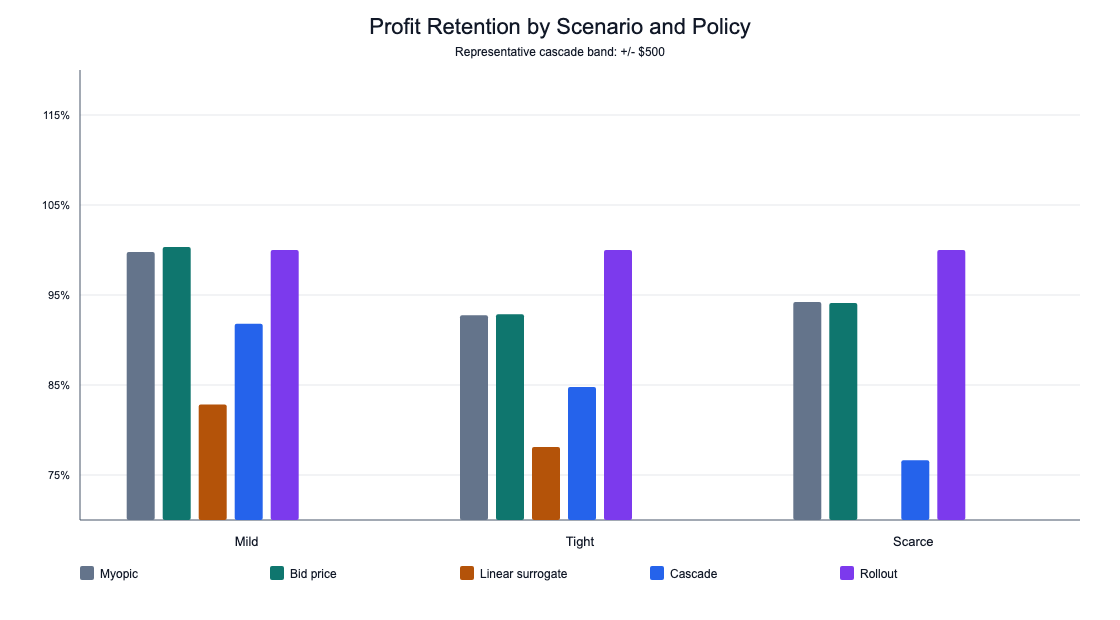
\includegraphics[width=\linewidth]{figures/profit_retention_by_policy.png}
\caption{Profit retention by policy.}
\label{fig:profit-retention}
\end{figure}

\begin{figure}[t]
\centering
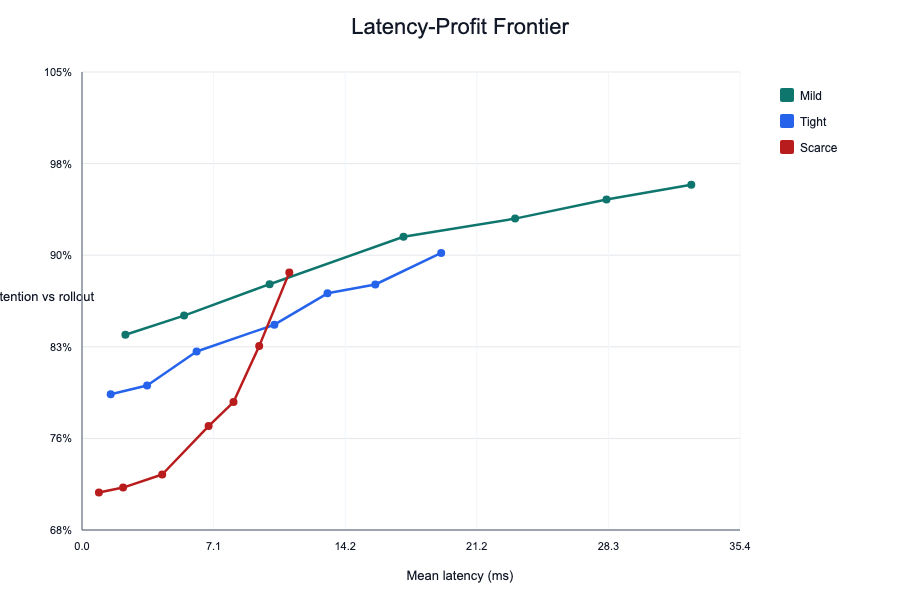
\includegraphics[width=\linewidth]{figures/latency_profit_frontier.png}
\caption{Latency-profit diagnostic frontier.}
\label{fig:latency-frontier}
\end{figure}

\subsection{Operational Feasibility Ablation}

We reran the standard preset with individual feasibility features disabled.
These are sensitivity tests, not recommended benchmark settings, and we keep
them on the cheaper standard preset because each toggle multiplies total run
count. Table \ref{tab:ablation} reports the change in myopic profit relative to
the full-feasibility benchmark. The result is large: removing appointment
windows raises myopic profit by 124.3 percent in \texttt{tight} and 194.0
percent in \texttt{scarce}; removing HOS raises myopic profit by 115.5 percent
and 154.5 percent in the same scenarios. Thus, a benchmark that omits these
constraints can make simple fast policies look much stronger than they are
under operational feasibility.

\begin{table}[t]
\centering
\caption{Standard-preset feasibility ablation. Full profit is the
full-feasibility myopic profit. Other columns report profit change after
disabling one or more feasibility features.}
\small
\begin{tabular}{lrrrrrr}
\toprule
Scenario & Full & No reach & No windows & No HOS & No yard & Minimal \\
\midrule
\texttt{mild} & \$1.083M & +28.2\% & +58.3\% & +57.9\% & +25.9\% & +67.3\% \\
\texttt{tight} & \$0.867M & +35.1\% & +124.3\% & +115.5\% & +32.5\% & +144.9\% \\
\texttt{scarce} & \$0.718M & +30.9\% & +194.0\% & +154.5\% & +27.9\% & +218.6\% \\
\bottomrule
\end{tabular}
\label{tab:ablation}
\end{table}

Pickup reach and yard delays also matter, but primarily as cost and time
frictions. Removing them raises myopic profit by roughly 26--35 percent across
the three scenarios. The all-disabled ``minimal feasibility'' variant is a much
easier problem: in \texttt{scarce}, myopic profit rises from \$0.718M to
\$2.288M. This supports the benchmark's central design choice: profit and
latency should be reported together with operational feasibility metrics.

\section{Discussion}

The central benchmark claim is that feasibility changes what is being measured.
The ablation results show that appointment windows and HOS constraints change
the benchmark regime by more than the current differences among several
reference policies. A policy that looks attractive under aggregate state-level
availability can create pickup-window misses, excess HOS rest, or yard-delay
exposure once individual truck feasibility is considered.

The full-feasibility policy table adds a second lesson. In v0.2, simple
policies are surprisingly competitive, and the representative cascade is not.
This is not a contradiction of the ablation result. It is a diagnosis of the
current benchmark economics. Accepted-but-unserviceable tenders are mostly
recorded as feasibility events rather than charged as service failures;
terminal truck position has little carryover value at the end of a 72-hour
horizon; and the demand process has limited temporal structure. These choices
make it hard for future-aware policies to separate from immediate-margin
policies.

For v0.3, the highest-leverage changes are therefore not longer runtimes by
themselves. The benchmark should first add explicit service-failure penalties
for accepted-but-unserviceable tenders, terminal value for end-of-horizon truck
positions, and temporal demand waves that make repositioning valuable. It
should also strengthen the quality anchor by reporting retention versus both
rollout and the best simple baseline, and by adding a hindsight realized-seed
diagnostic bound. Finally, the cascade thesis should be tested with a stronger
nonlinear surrogate before drawing conclusions about selective escalation.

\section{Limitations}

FreightBidBench v0.2 is not a production dispatch simulator. It uses synthetic
loads, public calibration, simplified HOS clocks, state-level geography, and
reference Python latency. It does not model road closures, traffic, weather,
team drivers, split sleeper rules, maintenance, customer-specific facilities,
or private tender distributions.

It is also not yet validated as a community benchmark in the strongest sense.
The current policy set is author-implemented, the surrogate baseline is linear,
and the generated tender distribution has not been tested against held-out
private tender aggregates. A stronger benchmark release should include
external policy submissions or stronger nonlinear baselines, calibration checks
against partner or held-out aggregate data, scenario axes beyond fleet
scarcity, and a realized-seed hindsight bound so rollout retention is anchored
above by a diagnostic ceiling.

\section{Reproducibility}

The benchmark release is designed around command-line reproduction rather than
manual notebook execution. Every benchmark run writes a manifest containing the
benchmark version, scenario-configuration version, policy-set version, command,
Python version, source inputs, scenarios, seed pairs, default policies, cascade
policy, evaluated policies, cascade bands, label limit, evaluation load limit,
feasibility-layer version, output file paths, and row counts. Benchmark
submissions should include the manifest and all summary CSVs.

The release artifact is identified by Git tag \texttt{v0.2.1} at
\url{https://github.com/aswincsekar/freightbidbench}, pinned to commit
\texttt{c0a385c1e269afe4efa4cfa1ca9afa6e7d37ca14}. Reproduction should start
from:
\begin{verbatim}
git checkout v0.2.1
\end{verbatim}

The v0.2.1 paper reference run is:
\begin{verbatim}
python3 scripts/run_freightbidbench.py --preset paper \
  --output-dir benchmark_runs/paper_v02
\end{verbatim}

Figures are generated from the resulting CSVs with:
\begin{verbatim}
python3 scripts/plot_freightbidbench.py --run-dir benchmark_runs/paper_v02
\end{verbatim}

Paired policy deltas are generated with:
\begin{verbatim}
python3 scripts/analyze_policy_deltas.py --run-dir benchmark_runs/paper_v02
\end{verbatim}

The current reference manifest is:
\begin{verbatim}
benchmark_runs/paper_v02/freightbidbench_manifest.json
\end{verbatim}

The standard feasibility ablation suite can be reproduced with:
\begin{verbatim}
python3 scripts/run_feasibility_ablation_suite.py --preset standard \
  --output-dir benchmark_runs/feasibility_ablations_standard
\end{verbatim}

\section{Conclusion}

FreightBidBench provides a public, reproducible testbed for real-time truckload
bid acceptance under operational feasibility. The v0.2 result is a calibration
result: benchmarks that omit appointment windows, HOS clocks, and individual
truck feasibility can substantially misstate policy performance, while the
current full-feasibility environment makes simple policies near-Pareto and
shows that the finite rollout teacher is a reference policy rather than a
reliable upper bound. This gives the benchmark a clear next step. Future
latency-quality claims should build on stronger service-failure economics,
terminal value, temporal demand structure, a realized-seed hindsight diagnostic
ceiling, and stronger teacher and surrogate baselines.

\bibliographystyle{plainnat}
\bibliography{references}

\end{document}
